\chapter{Brain-computer interfaces}
\label{sec:bci}
\todo{consistently terminology individuals with severe
speech and physical impairments (SSPI)}
\todo{uniform vsa condition vsa setting}
\todo{are all acronyms defined/Acro corectly used in chapters?}
\todo{footnot skips a page in wcble chap}


People with \ac{sspi} due to neurodegenerative disease, stroke, traumatic brain or spine
injury become entirely reliant on caregivers or family members in their day-to-day
routine.
Wouldn't it be great if we could help them regain some quality of life by making them
more independent?

The most basic ability any independent human being needs is interaction with their
environment.
In its core essence, this is the ability to communicate intentions, emotions,
frustrations, or thoughts such that they might be acted on.
For an able-bodied person, physical interaction happens through body movements, while
communication is usually done through speech and body language.
Both require sending signals through the body's nervous system to control muscles.
Not everyone has this capability.

The key problem for severely paralyzed individuals is that the mind wants to go where the
body cannot follow.
Couldn't we, therefore, design a system that directly interacts with the mind?
This system can then form an interface between the mind and any kind of technology, like
a robot arm or speech synthesizer, interacting with the world on the user's behalf.
Such a device is the \ac{bci}\footnote{Sometimes also termed brain-machine interface
(BMI) when coupled to a physical actuator, like a robot arm or an exoskeleton.
The term \ac{bci} is usually preferred for assistive technology and communication
devices.}, a system that directly couples actions in the `real world' to the mental state
of the user.

Starting in the 1970s from methods to establish basic communication from minimal brain
activity (yes/no, left/right, \ldots)~\cite{Wolpaw2002}, \acp{bci} have gradually evolved
into sophisticated interaction schemes that restore or enhance many capabilities by
bypassing defective parts of the nervous or muscle system.
By now, classic \acp{bci} methods are starting to mature outside the lab setting and can
be used as assistive communication technology by individuals with \acl{sspi}.
speech~\cite{Wolpaw2018,Milekovic2018}.
Impressive cutting-edge experimental examples include a brain-spine interface allowing a
paraplegic individual to walk again~\cite{Lorach2023}, a \ac{bci} translating internal
speech to a facial avatar speaking the imagined text~\cite{Metzger2023}, and fast
communication through decoding imagined handwritten symbols~\cite{Willett2021}.
Recently, the idea has also gained popular traction through Elon Musk's
NeuraLink~\cite{Musk2019} initiative, which imagines a multipurpose \ac{bci}.

In general, devices processing direct inputs from the central nervous system are useful
for rehabilitation and medical diagnosis or treatment.
Additionally, they bring a new paradigm to human-computer interaction, especially when
paired with virtual or augmented reality~\cite{SiMohammed2017}.
Ultimately, they have always been especially promising as assistive technology for
people limited in their communication ability.
It is this \ac{bci}-controlled communication where our focus lies, as it offers a
transformative means for individuals with severe motor impairments to regain functional
independence to write and speak through assistive technology.
This allows them to talk to their loved ones and caregivers, exercise hobbies, and makes
many aspects of daily life more accessible.

\section{A direct interface to the brain}
\todohsm{make less verbose}

Simply put, a \ac{bci} records the user's brain activity, extracts some relevant output
from this brain activity, and couples this output to a function of a device as
illustrated in \cref{fig:bci/loop}.
Optionally, the user can then observe the action of the device and adapt their behavior
or brain activity accordingly, closing the loop\footnote{\textcite{BCISociety2024} has
recently formalized this into the following definition: \it``A brain-computer interface
is a system that measures brain activity and converts it in (nearly) real-time into
functionally useful outputs to replace, restore, enhance, supplement, and/or improve the
natural outputs of the brain, thereby changing the ongoing interactions between the
brain and its external or internal environments.
It may additionally modify brain activity using targeted delivery of stimuli to create
functionally useful inputs to the brain.''}.

\fullpagefig[topleft]{%
  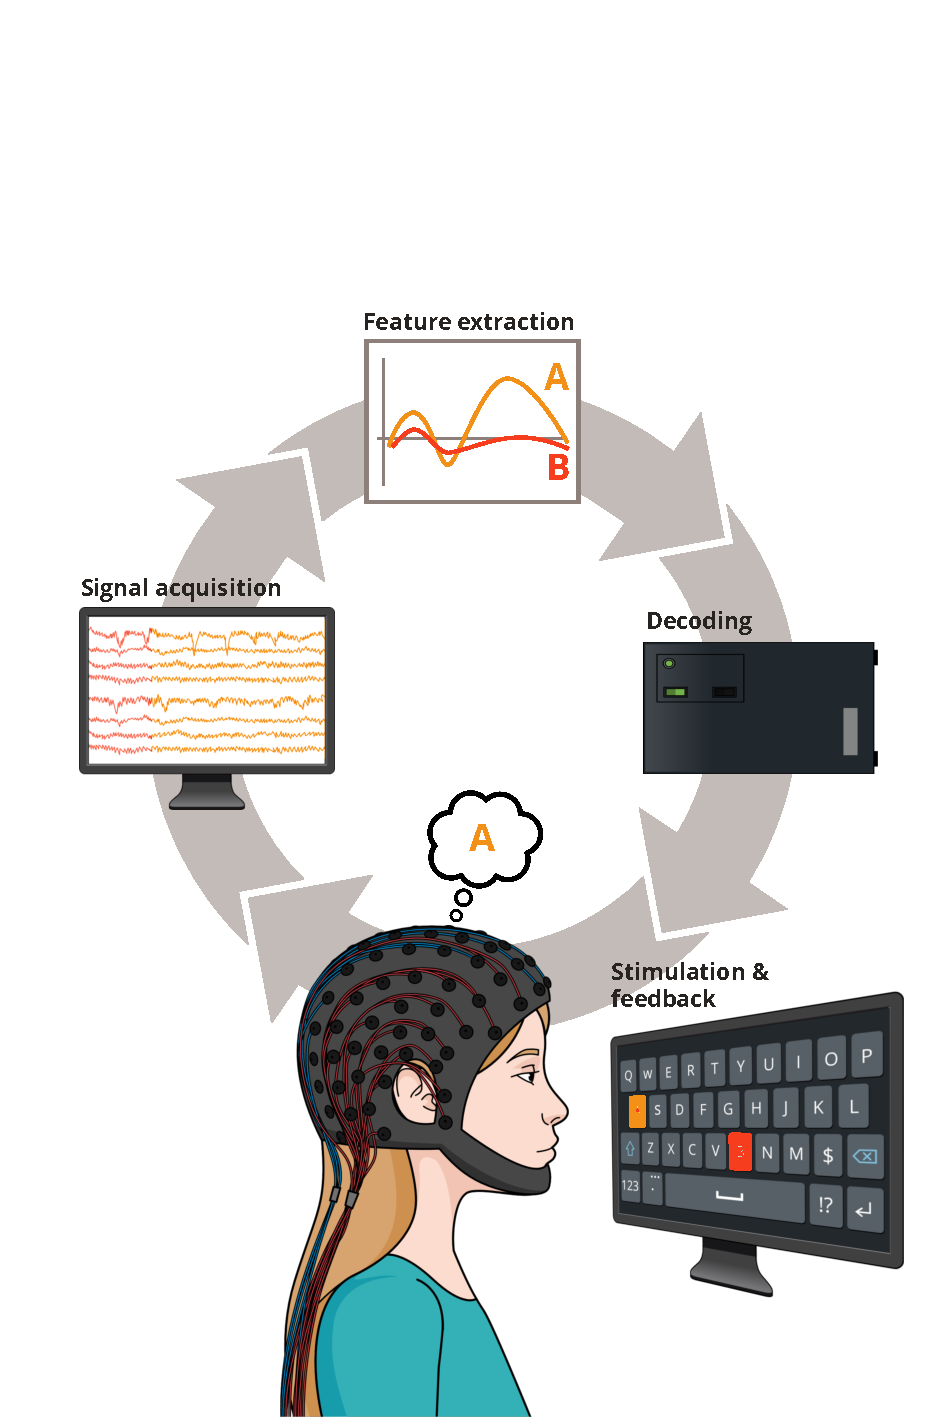
\includegraphics[width=\fullpagefigwidth]{figures/bci/bci_loop.pdf}
}{%
  The \acs{bci} loop.
}{%
  The \ac{bci} loop.
  The user interacts with the \ac{bci} via a specific paradigm, in this case involving
  visual stimulation.
  Electrical neural signals are recorded, and neurophysiological features related to the
  paradigm are extracted.
  Using machine learning, a decision can then be made based on these features, which can
  be presented back to the user.
  In a closed-loop \ac{bci}, this feedback allows the user to adapt to the \ac{bci}.
}{fig:bci/loop}

Let's break this definition down and focus on its separate parts.
First of all, we need to identify a signal that is a direct representation of what is
going on in the brain.
Multiple signals can be recorded from the brain, including blood flow and magnetic or
electrical activity.
For several reasons laid out in \cref{sec:bci-recording}, the electrical modality is
especially interesting.

The recorded brain activity forms only one part of the interaction scheme presented in
\cref{fig:bci/loop}.
It would make little sense to start digging around at random in all the brain activity
to try to extract the desired output.
Instead, it would help greatly if we knew which specific activity to look for.
A \ac{bci} operates according to a specified \emph{paradigm}, which defines the method
by which interaction is conducted.
This usually means that the user is instructed to perform a specific task, like
attending a specific flickering stimulus.
We can now exploit background knowledge from prior neuroscientific research to couple
specific activity in the brain to specific information or actions we want to convey via
the \ac{bci}.
The brain signal now \emph{modulates} this information.
In turn, the detection of this signal can be coupled to an action, like typing the
intended letter A or B in \cref{fig:bci/loop}.
The \ac{bci} paradigm comprises the manner of stimulation (if applicable) and the exact
task performed by the user, and is often closely linked to the manner of feedback in the
case of a closed-loop system.
As shown in \cref{sec:bci/paradigms}, there is a wide variety of \ac{bci} paradigms
based on different systems in the brain.

The previous points to another component of a successful \ac{bci}: the specific brain
signatures related to our paradigm need to be identified within the recorded activity.
The electrical activity of the brain is relatively weak compared to that of the
environment around us, containing electronic devices and other sources of interference.
Furthermore, the brain is continuously processing information and carrying out
`background tasks,' all of which generate their own brain activity.
On the other hand, the activity of interest often originates from a specific region or
network within the brain.
This activity might not easily be discerned from all other brain and environmental
activity.
Compare this to trying to listen to a single speaker at a noisy party where everyone is
shouting over each other.
Some obvious sources of interference can be easily filtered out by \emph{preprocessing}
(see \cref{sec:bci/preprocessing}) and by choosing the correct representation of the
signal (i.e., \emph{feature extraction}), but the problem of retrieving or
\emph{decoding} only the relevant signal is generally hard.
Nevertheless, we can attempt to solve it through supervised machine learning.
Useful information that is encoded in the brain signal by the paradigm can be retrieved
from it by the decoder and interpreted in function of the desired \ac{bci} output.
\Cref{sec:bci/decoding} takes a closer look at some common decoding techniques.

Finally, the loop can be closed by coupling this to a device or actuator.
There are two aspects to this.
On the one hand, the \ac{bci} gains its function by allowing the user to interact with
their environment.
For a communication system, this means coupling the decoded information to, e.g., a
virtual keyboard or speech synthesizer.
On the other hand, the actions performed by the \ac{bci} can themselves alter the user's
cognitive state or brain activity, creating an adaptive system.
A direct form of closed-loop \ac{bci} is the use of a neurostimulator.
Examples of this are deep brain stimulation to mitigate the symptoms of Parkinson's
disease, or the cochlear implant as a hearing prosthesis.
More indirectly, modulation can be achieved by sensory stimulation.
This involves specific, paradigm-related sensory input, like tactile feedback for
movement \ac{bci}~\cite{Flesher2021}, or simply presenting selected actions back to the
user.
The user's brain will then adapt through reinforcement learning, causing changes in
behavior or strategy.
Neuroplasticity, the brain's ability to adapt and reinforce specific neural pathways,
can have a positive impact on \ac{bci} performance and gives rise to rehabilitation
applications.

To summarize, a \ac{bci} can facilitate direct interaction with the central nervous
system.
To do this, information is modulated in the brain signal according to the \ac{bci}
paradigm by stimulating the user or having them perform a task.
Their brain signal is subsequently recorded and preprocessed to clean it.
Relevant features that contain aspects of the modulated signal are extracted, and the
modulated information is retrieved by the decoder, a machine learning model.
This information can then be acted on, and the loop is closed if this action affects the
user.
Let us take a look at each of these elements separately in the next section.

\section{Recording technologies}
\label{sec:bci-recording}

The brain's activity can be recorded using various neuroimaging technologies.
These can range from brain scans~\cite{Weiskopf2004} using functional magnetic resonance
imaging (fMRI) to more portable technologies like acoustic signals obtained by
functional ultrasound imaging (fUS)~\cite{Zheng2023} and functional near-infrared spectroscopy
(fNIRS)~\cite{Borgheai2020}.

The technologies above all measure blood flow (the hemodynamic signal), which only
indirectly reflects brain activity.
This signal reacts too slowly to reflect the real-time activity that is of interest in
\ac{bci} for communication, and it carries little information other than the brain
region from where it is originating.

A better candidate is the neuronal electrical activity.
The brain contains 86 billion neurons, which are highly interconnected cells that are
the smallest units of information processing.
The \emph{action potential} and its related \emph{postsynaptic potential} are electrical
pulses occurring when a neuron receives input from another neuron and is activated.
The firing of a neuron, or the combined firing of groups of synchronized neurons, thus
generates an electrical field in and near the brain, which can be measured using
electrodes.
The related discipline is \emph{electrophysiology}.

Because of the desirable high temporal resolution~\cite{Easttom2021} and practicality of
electrophysiology, we will focus only on methods to record electromagnetic activity
originating from neuronal action potentials and postsynaptic potentials.
The magnetic field of the brain can be measured using magnetoencephalography
(MEG)~\cite{Mellinger2007}.
While MEG is non-invasive and results in high-quality signals, the necessary equipment
is rather expensive and impractical.
Recent advances have been made using optically pumped magnetometers
(OPM-MEG)~\cite{Wittevrongel2021}, but this technology still falters outside of lab
conditions.
As a consequence, the \ac{bci} field relies heavily on the electrical activity of the
brain.

\subsection{Invasive electrophysiology}

The \emph{invasiveness} of the technology forms an important concept in determining its
suitability for a given application and user.
As illustrated in \cref{fig:bci/recording}, invasive electrodes can often measure a
very specific brain region and can result in better signal quality, at the cost of the
risks involved with brain surgery.

\fullpagefig[topleft]{%
  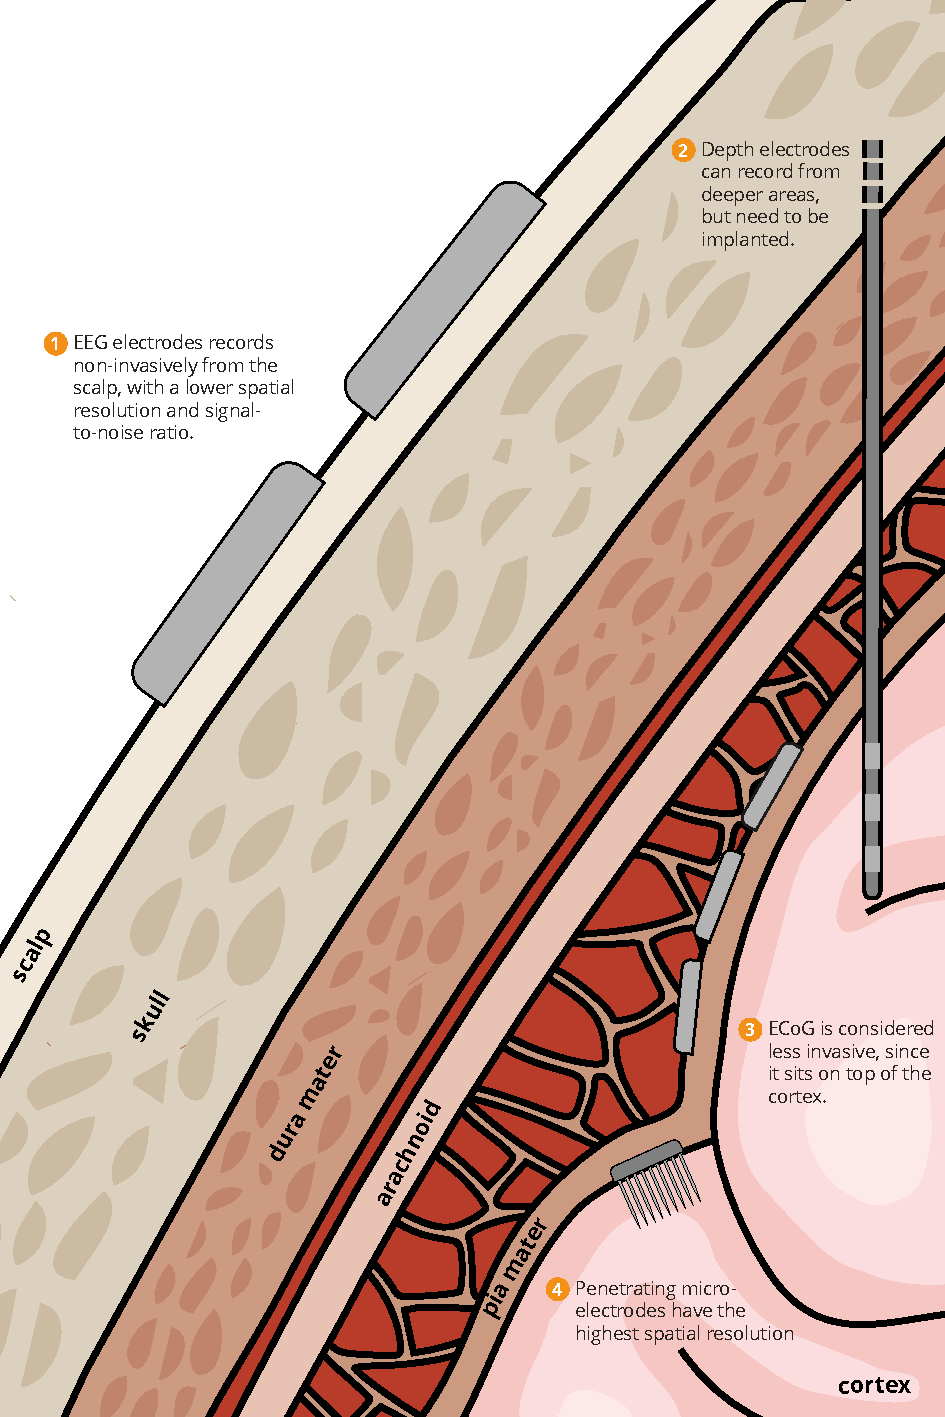
\includegraphics[width=\fullpagefigwidth]{figures/bci/recording_modalities.pdf}
}{%
  Various electrophysiology recording technologies.
}{%
	Various electrophysiology recording technologies and their respective position in a
	cross-section of the skull.
	There is a trade-off between invasiveness and spatial resolution.
}{fig:bci/recording}

Specifically, invasive methods are less noisy and come with an increased \emph{spatial
resolution}, meaning they can extract a signal from a specific brain region or even a
set of neurons of interest.
This makes it easier to retrieve a signal with a known origin from the brain, which
might be leveraged by the paradigm to modulate information.
Generally, microelectrodes penetrating the cortex are considered to have the highest
spatial resolution.
These are needles with a diameter smaller than 10µm and one or multiple electrodes that
extend several millimeters into the cortex.
Microelectrodes can measure the Local Field Potential (LFP), the extracellular potential
of a small group of neurons, or even intracellular single neuron action potential
spikes.
They come in single-electrode form, or, more popularly, in microelectrode arrays.
Well-known examples are the Utah array~\cite{Maynard1997}, the more recent NeuraLink
implant~\cite{Musk2019}, and IMEC's Neuropixels 2.0~\cite{Steinmetz2021}.

Larger implanted electrodes are referred to as intracranial \ac{eeg} (i\ac{eeg}).
Depth electrodes, like those found in in stereo-\ac{eeg}, can be used for \ac{bci}~\cite{Wu2024}
 and other applications, like closed-loop adaptive control for Deep Brain Stimulation to mitigate Parkinson's disease
symptoms~\cite{Arlotti2018}.
Depth electrodes are longer rods with multiple electrodes that can extend deeper into
the brain.
Since these still penetrate the cortex, electrodes that sit on top of the cortex are
more popular, as they are considered less invasive.
\Ac{ecog} is a powerful method with many applications in \ac{bci}~\cite{Schalk2011} and
epilepsy diagnosis.
Newer developments like micro-ECoG (µECoG)~\cite{Shokoueinejad2019}, with a higher
number of smaller electrodes per surface area, allow for more precise measurements.

Some impressive recent breakthroughs in speech and motor \ac{bci} for communication have
been realized using invasive microelectrode arrays~\cite{Willett2021} and
$\mu$\Ac{ecog}~\cite{Metzger2023}.
Furthermore, recent advances in recording technology focus on improving implant
durability and resolution~\cite{Steinmetz2021}, and on balancing the invasiveness
tradeoff by finding new, minimally invasive ways to record from closer to the cortex.
The Synchron Stentrode~\cite{Mitchell2023}, for instance, can be delivered through the
bloodstream via a catheter, removing the need for open brain surgery.
Nevertheless, surveys~\cite{Huggins2011, Huggins2015, Branco2021} in different
potential communication \ac{bci} user groups consistently show that non-invasive
technology is preferred over implanted electrodes, unless the added value of invasive
BCI is sufficiently large~\cite{Kageyama2020}.
This provides justification for focusing part of the current research effort on
non-invasive BCI.

\subsection{\Acl{eeg}}

\Ac{eeg} is the de facto non-invasive electrophysiology standard in clinical neurology
practice as well as in \ac{bci} research.
Developed since 1924~\cite{Berger1929}, it is cheap and relatively practical and offers
great temporal sampling resolution up to thousands of Hz.
\Ac{eeg} measures the electrical potential over time at a given electrode relative to a
reference electrode in volts (V), often on the scale of microvolts ($\mu$V).
As it is easily applicable on the outside of the scalp, many practical consumer-grade
\ac{eeg} headsets exist in the form of (often wireless) electrode caps or helmets.
Current consumer systems sometimes feature dry electrodes, but clinical and research
systems often use active electrodes with preamplifiers and electrolyte gel to reduce
impedance for improved signal quality, which slightly decreases practicality, since they
require a trained individual to properly administer.
Nevertheless, it is the most accessible \ac{bci} technology for both users and
researchers.

The major drawback of \ac{eeg} is its poor spatial resolution~\cite{Ferree2001}.
Since they sit on the outside of the scalp, electrodes are large and distant relative to
the neurons in the cortex they ought to measure.
Furthermore, the layers of skull and cerebrospinal fluid in between can attenuate the
signal and cause volume conduction~\cite{Broek1998}, which results in electrodes
measuring a mixture of activity from sources elsewhere in the brain.
This also has a negative effect on spectral resolution.
The noise problem mentioned earlier is also prominently present in \ac{eeg} recordings.
In addition to picking up brain activity other than that of the region of interest,
\ac{eeg} also records other artifacts from the environment, the power supply, nearby
electrical equipment, or the user's muscle movements~\cite{Urigueen2015}.
Combined, this means \ac{eeg} is inherently noisy.

Despite its noisy nature, \ac{eeg} is the recording methodology of choice for our
\ac{bci} because of its wide acceptance by users.
To counteract the noise present in our recording, we must on the one hand evoke strong,
informative brain activity using a suited \ac{bci} paradigm, and on the other hand pick
a suited decoder which can isolate the signal of interest and filter out the noise.


\section{Paradigms}
\label{sec:bci/paradigms}

\subsection{Active \& passive \acsp{bci}}

The \ac{bci} paradigm~\cite{Xu2021,Neeling2019} is the key to translating brain activity
into useful output actions, since it defines which neural responses will be elicited and
captured as features.
A paradigm can be loosely seen as \emph{a way of interacting with the \ac{bci}}.
According to \textcite{Zander2011}, they can be arranged by their reliance on external
stimulation and the engagement of the user as shown in \cref{fig:bci/paradigms}.

\fullpagefig{%
  \sffamily
\begin{tikzpicture}[
    scale=\textwidth/3cm,
  ]
  \useasboundingbox (-1,-1.25) rectangle (1,1);
  \pgfmathsetmacro{\margin}{.1}
  \pgfmathsetmacro{\center}{.5+.5*\margin}
  \pgfmathsetmacro{\textspacing}{.15}
  %\begin{scope}[shift={(1,1.2)}]
    % Draw axes
    \draw[darkgray, very thick, <->] ({-(1+\margin)}, 0) -- ({1+\margin},0);
    \draw[darkgray, very thick, <->] (0,{-(1+\margin)}) -- (0,{1+\margin});

    % Draw rectangles
    \draw[draw=accent1, fill=white, very thick] ({-\margin}, \margin) rectangle (-1,1);
    \draw[draw=accent2, fill=white, very thick] (\margin, \margin) rectangle (1,1);
    \draw[draw=accent3, fill=white, very thick] (-1, {-\margin}) rectangle (1,-1);

    %% Add text
    \node[color=accent1, align=left,font=\bfseries, anchor=north west, inner sep=2pt] at  (-1,1){active};
    \node[color=accent2, align=left,font=\bfseries, anchor=north east, inner sep=2pt] at  (1,1){reactive};
    \node[color=accent3, align=left,font=\bfseries, anchor=south west, inner sep=2pt] at  (-1,-1){passive};

    \node[color=darkgray, align=center,font=\bfseries, anchor=north] at
    (0,{-(1+\margin)}) {passive\\participation};
    \node[color=darkgray, align=center,font=\bfseries, anchor=south] at
    (0,{1+\margin}) {active\\participation};
    \node[color=darkgray, align=center,font=\bfseries, anchor=east] at ({-(1+\margin)}, 0) {stimulus\\independent};
    \node[color=darkgray, align=center,font=\bfseries, anchor=west] at ({1+\margin},0) {stimulus\\dependent};

    %% Text in rectangles
    \node[align=center,font=\small, color=muteblack] at ({-\center}, {\center+1.5*\textspacing}) {motor\\imagery};
    \node[align=center,font=\small, color=muteblack] at ({-\center}, {\center}) {imagined\\speech};
    \node[align=center,font=\small, color=muteblack] at ({-\center}, {\center-1.5*\textspacing}) {neurofeedback};

    \node[align=center,font=\small, color=muteblack] at ({\center+\textspacing}, {\center+\textspacing}) {P300};
    \node[align=center,font=\small, color=muteblack] at ({\center+\textspacing}, {\center-\textspacing}) {SSVEP};
    \node[align=center,font=\small, color=muteblack] at ({\center-\textspacing}, {\center+\textspacing}) {cVEP};
    \node[align=center,font=\small, color=muteblack] at ({\center-\textspacing}, {\center-\textspacing}) {mVEP};

    %% More text
    \node[align=center,font=\small, color=muteblack] at ({\center}, {-\center+\textspacing}) {error\\potentials};
    \node[align=center,font=\small, color=muteblack] at ({-\center}, {-\center+\textspacing}) {attention and \\ workload detection};
    \node[align=center,font=\small, color=muteblack] at ({-\center}, {-\center-\textspacing}) {clinical neuroimaging \\ and monitoring};
    \node[align=center,font=\small, color=muteblack] at ({+\center}, {-\center-\textspacing})  {emotion \\ detection};
  %\end{scope}
\end{tikzpicture}

}{%
  Overview of \acs{bci} paradigms.
}{%
  A \ac{bci} paradigm defines which brain activity will be used for control.
  They can be categorized in active, reactive and passive paradigms, depending on their
  reliance on external stimulation and active participation required from the user.
  Adapted from~\textcite{Muehl2014}.
}{fig:bci/paradigms}

Paradigms that require little active participation from the user, like redirecting
attention or initiating imagined actions, are classified as \emph{passive \ac{bci}}.
From the user's point of view, this concept is probably the most attractive, since their
cognitive state would be inferred from just their brain activity.
However, without active user participation, it can be hard to establish reliable
communication or control.
Therefore, passive \ac{bci} are currently more suited to tasks like emotion or affect
monitoring~\cite{Torres2020,Libert2019, Muehl2014}, workload monitoring~\cite{Zanetti2021},
or, more dependent on stimulation, error detection~\cite{SiMohammed2020}.
It also has clinical applications in the form of neurofeedback~\cite{Hammond2011}.
Nevertheless, active participation facilitates training data collection for supervised
machine learning, since the conditions can be more easily controlled by the user or the
stimulation.

Paradigms requiring high active participation can be split up into \emph{active
\ac{bci}} and \emph{reactive \ac{bci}}.
Active \ac{bci} paradigms encode endogenous activity initiated by the user, such as
imagined movement or imagined speech.
These tasks can encode complex information, but current non-invasive communication
methods often limit the considered domain to a few movement directions to control a
cursor, or a few words~\cite{Panachakel2021}.
Invasive recordings are necessary for decoding more complex encoded activities like
natural speech~\cite{Metzger2023} or meaningful motor trajectories, like handwritten
symbols~\cite{Willett2021} or sign language~\cite{Branco2017}.
Active paradigms are also subject to large inter-subject variability due to the
complexity of the performed tasks.
They might require extensive user training and are sensitive to correct task
instruction.
Imagined speech or movements can be performed in a multitude of ways, which can each
have different neural representations for separate individuals.
This can make it hard to adapt the \ac{bci} to specific individuals, causing poor
performance and giving rise to the concept of \ac{bci} illiteracy~\cite{Allison2010}\footnote{%
Recently, the concept of BCI illiteracy is increasingly being seen as outdated.
Instead of attributing poor performance to the user's inherent limitations, critiques
point out that the issue lies more with the design of the systems themselves.
BCI systems often fail to account for individual variability in brain anatomy and
cognitive strategies.
As a result, what has been labeled as `illiteracy' may, in fact, be a reflection of
systems that are not flexible enough to adapt to different users.
This perspective shifts the responsibility to the individual, rather than recognizing
that better, more adaptive systems could overcome many of these performance challenges,
thus standing in the way of progress.
Moreover, the term `illiteracy' itself carries negative connotations, implying a user
deficiency that reinforces normative assumptions, when in reality, a more inclusive
approach to design could enhance BCI accessibility for a wider range of
individuals.
This evolving view calls for a reframing of the problem, focusing on improving the
adaptability of BCIs rather than labeling users as illiterate~\cite{Becker2022,Thompson2019}.}.

\subsection{Reactive \acsp{bci}}
Reactive \ac{bci} take another approach by providing a discrete set of sensory
stimulations towards which the user's attention can be directed.
Compared to active \ac{bci}, reactive paradigms can more easily induce fatigue due to
the constant stimulation.
These paradigms are also somewhat less intuitive compared to, e.g., speech, and their
expressive power is limited by how many different stimuli can effectively be presented
and attended to within a reasonable timeframe.
Nevertheless, reactive \ac{bci} work well with \ac{eeg} recordings, and, most
importantly, they work for most people~\cite{Allison2010a,Edlinger2014}.

Reactive \ac{bci} can be realized in multiple ways, depending on the stimulation used.
Some examples include the following:
In the steady-state somatosensory evoked potentials paradigm~\cite{Petit2021}, the user
can attend to one of multiple vibrotactile stimulations in different limbs, which
encodes the information of the attended limb in the brain signal.
In auditory paradigms, information can be modulated by the volume, tone, pitch, or
spatial origin of presented sounds, to which the user can attend~\cite{Kaongoen2017}.
Most common are the visual paradigms.
These can be more performant since they allow the user to use their visual system, one
of the most evolved sensory systems in humans.

The major visual paradigms rely on \ac{ssvep}, \ac{cvep}, oddball, and \ac{mvep} brain
responses.
In \ac{ssvep}, information is modulated by the frequency of a stimulus attended among
many that each flicker continuously at different frequencies~\cite{Chen2021}.
In \ac{cvep}, the stimuli flicker instead with distinct on-off patterns, which can be
correlated with the brain activity to retrieve the attended stimulus~\cite{Sun2022}.
Instead of stimulating all possible selections at once, the oddball paradigm stimulates
them one by one with single flashes~\cite{Pan2022}.
Since the times of stimulation of each target are known, and time-points at which an
attention signature is detected can be correlated to selected targets.
\Ac{mvep} is usually similarly time-modulated, but stimuli make sudden movements in
specific directions instead of flashing.
Information is then also carried by movement direction~\cite{Libert2021a,Libert2022}.

The \ac{bci} paradigms mentioned above can also be combined to gain performance.
Straightforward examples are activating or deactivating \ac{ssvep} stimulation with a
motor command~\cite{Neeling2019}, or combining multiple visual paradigms by stimulating
along multiple dimensions at once.
\textcite{Han2023} recently used this strategy, combining frequency and phase coding in
\ac{ssvep} with the \ac{mvep} and oddball paradigms to develop an efficient \ac{bci}
where one of 200 targets can be accurately selected with only 800ms of stimulation.

\section{Preprocessing}
\label{sec:bci/preprocessing}

\ac{eeg} preprocessing is a critical step in brain-computer interface (BCI) systems, as
it significantly improves the quality of the recorded data for subsequent analysis and
classification.
Common preprocessing techniques in BCI systems include rereferencing, band-pass and
notch filtering, and \ac{ica}.

Rereferencing is an essential first step, where the potential of each \ac{eeg} channel
is recalculated relative to a common reference point, such as the average of all
electrodes (common average reference) or a selected neutral set of electrodes.
This technique helps reduce noise common across all channels, improving signal clarity
and enhancing the accuracy of subsequent processing steps.

Band-pass filtering is then usually applied to isolate the frequency ranges of interest
by removing frequencies that are too high or too low to contain relevant neural signals.
Band-pass filters eliminate slow drifts and high-frequency noise, such as muscle
artifacts or environmental electrical interference, improving the \ac{snr}.
Additionally, notch filtering can be used to remove strong power line interference\footnote{%
Typically at 50Hz in Europe.}.
This interference can heavily contaminate \ac{eeg} recordings and even leak through when
outside the passband of a previous filter.
Notch filtering efficiently attenuates this narrowband noise without affecting the
surrounding frequencies.

Finally, to address artifacts like eye blinks and saccades that can significantly
distort the \ac{eeg} signal, \ac{ica} is performed~\cite{Delorme2007}.
\ac{ica} is a blind source separation technique that decomposes the \ac{eeg} data into
statistically independent components.
Components corresponding to eye movements, blinks, and other bodily or environmental
artifacts can be identified, either visually based on their characteristic topographies
and time courses, or statistically, and then removed.
This leads to cleaner data for subsequent processing, especially in the case of visual
\ac{bci} paradigms.
Since eye movement plays a role in the paradigm, it can strongly be present in the
signal and correlate with the task, forming a confounding factor for studying control
based solely on brain activity.

Together, these preprocessing steps ensure that only the relevant neural signals are
passed on to the feature extraction and classification stages in BCI applications,
improving the accuracy and reliability of the system.

\section{Decoders}
\label{sec:bci/decoding}

\subsection{Design principles}

After preprocessing and extracting features, machine learning algorithms can perform
\ac{bci} decoding.
Machine learning decoders use some training data for which the performed tasks are
known, and learn to recognize the activity elicited by the task in recorded data.
The training data can be either obtained from the \ac{bci} user themselves or from other
users.
In the first case, the user would perform a short calibration session before using the
\ac{bci}, where they are instructed to perform a known task.
This calibration session can be eliminated by training the decoder on preexisting
labeled data from other sessions and users, but this is harder due to the variability
between subjects and sessions.

If the goal is to eliminate the per-session calibration, one can also use a decoder
pre-trained on an existing dataset of the same task.
This is complicated by large variability in measured brain responses between subjects
and even between different sessions within the same subject~\cite{Guger2009,Saha2020}.
Therefore, pre-trained decoders must either be trained on a very large, diverse sample
of subjects, or some form of transfer learning must be applied.
Nevertheless, in practice, pre-trained models or models using transfer learning often
still require some per-session fine-tuning, which necessitates some calibration.
Instead, it is better to opt for keeping the calibration time as short as possible by
using an algorithm that can learn from very few training samples.
This can work well but requires strong regularization~\cite{VanDenKerchove2022}.

Decoder choice is heavily dependent on constraints set by the paradigm and the
application.
The number of output degrees of freedom, the serial or parallel nature of performed
tasks, and whether the paradigm is active or reactive, all need to be taken into
account.
One of these choices is whether to solve a \emph{regression} or \emph{classification}
problem.
In regression, a continuous output variable is predicted for a new sample, while
classification attempts to sort it into one of a set of discrete classes.
Regression can be useful in \acp{bci} for applications like mapping imagined movement to
an external robot arm.
For communication \acp{bci}, however, conveying information in a symbolic manner is
often of interest.
Many applications resemble virtual keyboards or map a user's actions to discrete words,
predefined actions, or letters for full control.
Hence, such problems often present themselves as classification tasks.

\subsection{Implementation \& evaluation}

\textcite{Lotte2018, Xu2021} present a relatively recent overview of state-of-the-art
classification algorithms for decoding.
Classic linear methods, such as \ac{csp} feature extraction for motor
imagery~\cite{Park2017} and \ac{cca} for \ac{ssvep}~\cite{Nakanishi2017}, and \ac{lda}
for \ac{erp} classification~\cite{Sosulski2022} still perform relatively well, given
some regularizing constraints or extensions.
Multi-linear techniques exploiting the tensor structure of neural signals are also
promising~\cite{Lotte2018}.
Riemannian Geometry~\cite{Barachant2014} is a popular and robust new strategy.
Furthermore, they lend themselves well to applications like adaptive
learning~\cite{Benaroch2021} or transfer learning~\cite{Zanini2017}.
Riemannian Geometry classifiers are often considered the current state-of-the-art.
Finally, deep learning~\cite{Bhuvaneshwari2021} is also sometimes considered, albeit
only when sufficiently large training datasets are available.
If decoders tailored to a specific user that keep the calibration session as short as
possible are of interest, not enough training data is available to properly train a deep
learning model.

Usually, a decoder makes a prediction for a given \emph{trial} while operating the
\ac{bci}.
A trial is the smallest unit on which a selection decision can be made, for instance,
one imagined movement or one repetition of flashing all targets in a visual \ac{erp}
\ac{bci}.
Accuracy is a valuable metric to assess decoder performance in the classification case.
Accuracy is calculated as the proportion of correct selections to all selections made.
It should be carefully interpreted in the presence of imbalanced data and always
compared to the random chance accuracy level in the presence of more than two possible
selections per trial.
Alternatively, \ac{rocauc} is also a measure of classifier predictive power but is more
suited for evaluation of classification of single epochs of data and in the presence of
imbalanced data, e.g., when comparing single \acp{erp}.
Higher \ac{rocauc} usually translates to a higher target selection accuracy.

Finally, an important concept in the evaluation of a \ac{bci} decoder, and of \acp{bci}
in general, is \ac{itr}.
\Ac{itr} reflects how fluently a \ac{bci} can be used for communication and can be
calculated as
\begin{equation}
  \text{\acs{itr}} = Q\left(\log_2N+P\log_2P+(1-P)\log_2\frac{1-P}{N-1}\right)
\end{equation}
\Ac{itr} is expressed in bits/s and is dependent on $N$, the number of different options
that can be selected per trial\footnote{Given that selections are independent of each
other. This formula requires some adaptations in the case of sequential or hierarchical
selection.}, $P$, the selection accuracy of the decoder, and $Q$, the number of trials
per second.
The parameters $N$, $P$, and $Q$ of this formula give us some insight into the building
blocks of a successful, high-\ac{itr} \ac{bci}.
To improve performance, we can aim to
\begin{enumerate*}[label={\arabic*})]
\item increase $N$ by selecting a paradigm and interface that offer a broad range of
informative selections per trial,
\item increase $P$ by engineering more performant machine learning methods for decoding,
and
\item increase $Q$ by selecting a paradigm that allows fast stimulation or responses.
\end{enumerate*}

\section{A case study: the visual oddball \acs{bci}}

The visual oddball paradigm is a \emph{reactive}, \emph{stimulus-dependent},
\ac{bci} paradigm with all the benefits and drawbacks.
Nevertheless, it can score relatively high on the \ac{itr} parameters established above.
The brain response of interest is the visual \ac{erp}, which can be accurately measured
and decoded from non-invasive \ac{eeg} signals with a relatively low computational
effort and short calibration time.
First established by~\cite{Farwell1988} in 1988, it is well supported by literature and
has been proven to work for those with \acl{sspi} in day-to-day home use~\cite{Wolpaw2018}.

\subsection{Stimulation paradigm}

One by one, visual elements on a computer screen are \emph{intensified} for a short
period of time by changing in color, brightness, or size.
Intensifications of different targets are usually 100-200ms apart and last for about
100ms~\cite{Sellers2006a}.
On each flash observed by the user, specific brain activity is elicited.
If one of these intensified elements is rare with respect to the others, i.e., it is the
\emph{odd-one out} or \emph{oddball}, this brain activity is altered.
A stimulus can be rare either due to its inherent properties like color or location.
Crucially, this is also the case if it is `marked' as rare by the user, e.g., by paying
explicit attention to only a given stimulus and not the others or counting how many
times it occurs.
If these visual elements represent letters, and we know the timing of the
intensifications of each letter, we can now establish communication by detecting for
which letter an oddball response was present in the brain signal at its time of
intensification.

\Ac{itr} in the oddball paradigm is optimized by intensifying multiple targets at once
in a row-column strategy and using a sequence of selections, giving rise to the classic
matrix speller of~\cite{Farwell1988}.
Other optimizations increase response \ac{snr}, like using flashing face images as
intensifications~\cite{Jin2012} or adding distinct colors and shapes to the
stimuli~\cite{Treder2011}.
The number of targets in a visual oddball \ac{bci} is limited by the crowding effect,
which imposes a limit on how close targets can be to each other while not distracting
the user's attention~\cite{Sellers2006a,Li2010}.
This may be overcome by making hierarchical selections of stimuli representing groups
of selections~\cite{Treder2010}.

Together with \ac{ssvep}, oddball paradigms are most frequently used in visual \ac{bci}.
There are, however, indications that users prefer oddball stimulation over \ac{ssvep},
which can cause eye strain and fatigue due to the continuous oscillatory stimulation of
all targets at once~\cite{Xu2021}.
Furthermore, \ac{ssvep} relies more on directing the gaze at the intended target than
oddball, detracting from the concept of control independent from muscle movement.

\begin{figure}[t]
  \centering
  \begin{subfigure}[t]{.45\textwidth}
  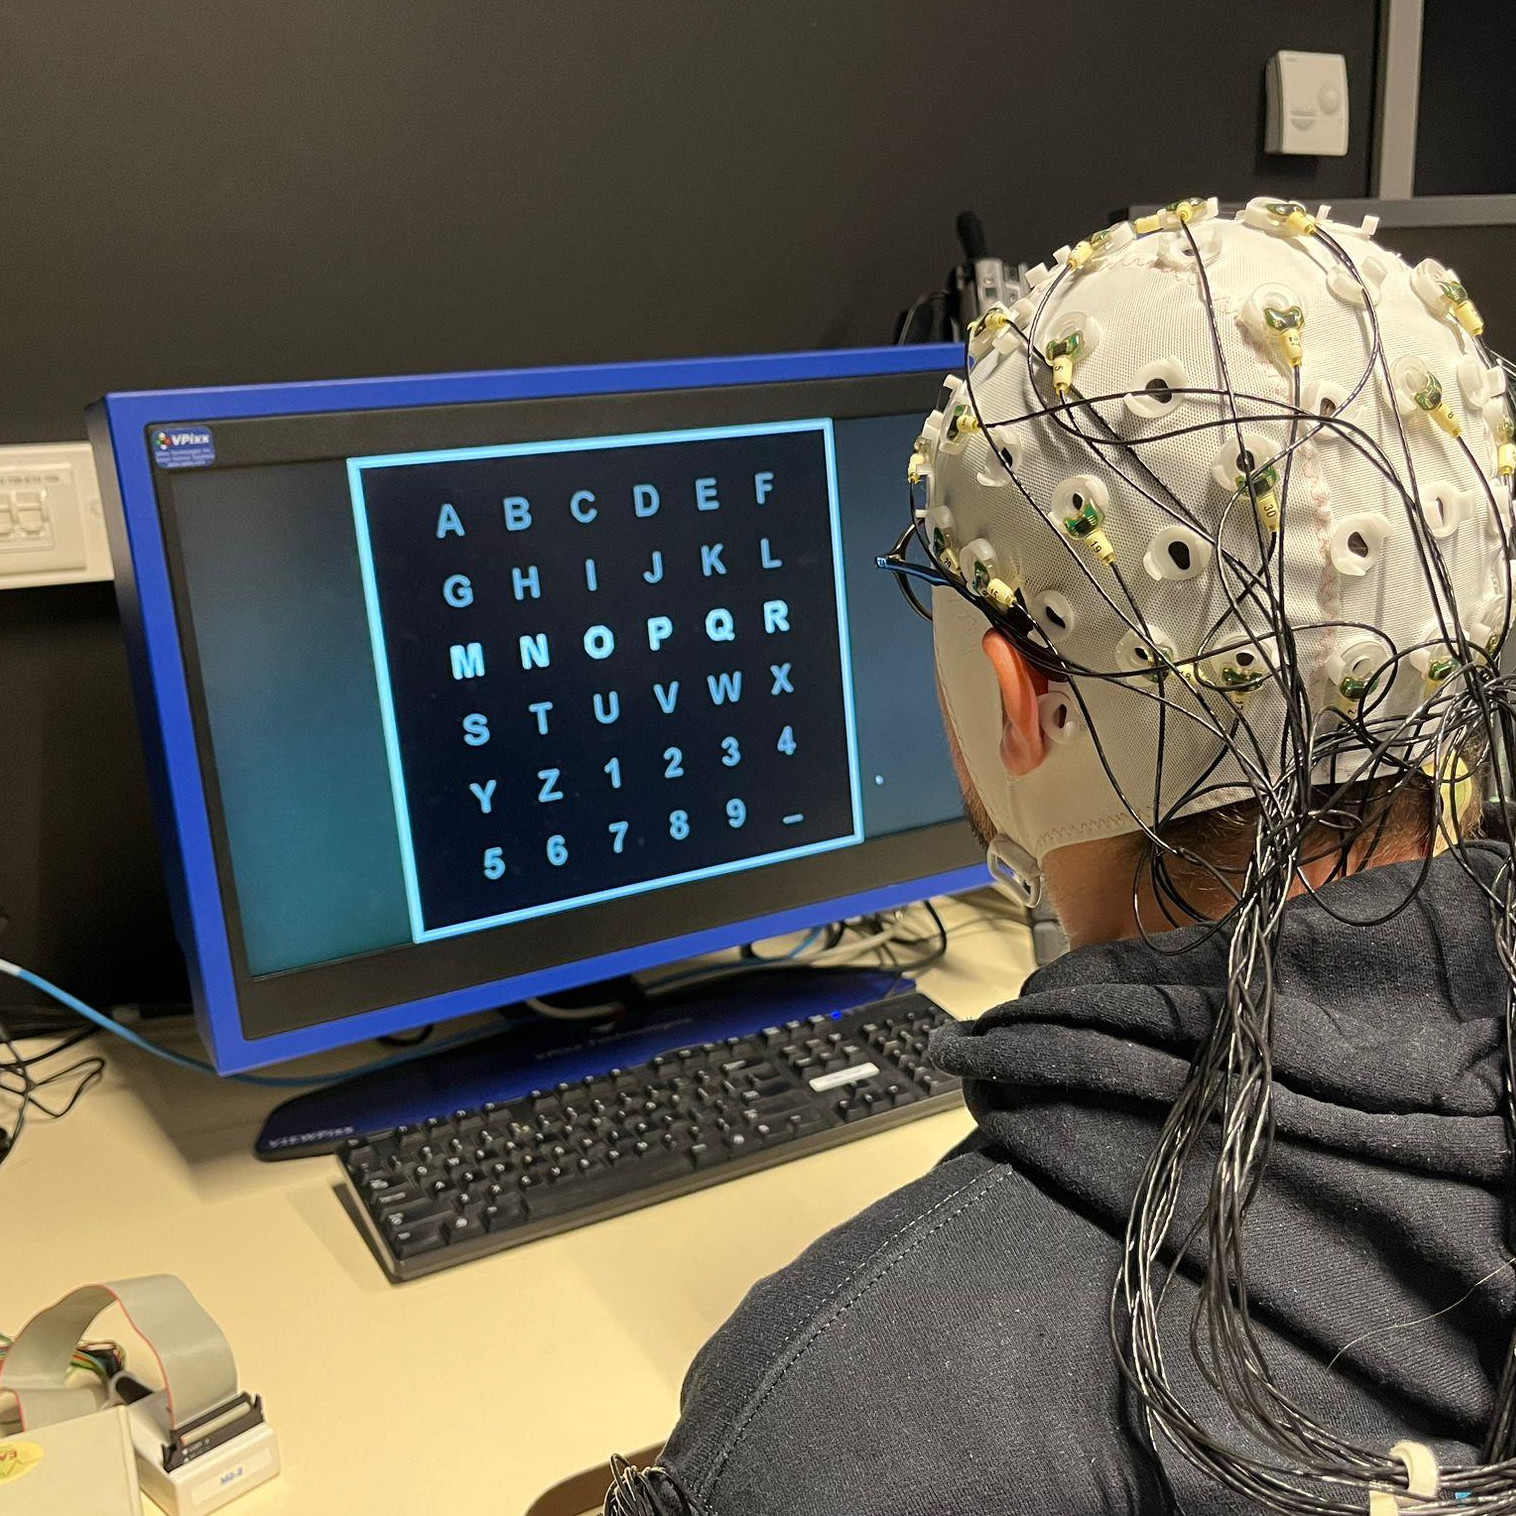
\includegraphics[width=\textwidth, height=\textwidth]{figures/bci/illustration}
    \caption{Stimuli are flashed while the \acs{eeg} is recorded.}
  \end{subfigure}\hfill%
  \begin{subfigure}[t]{.45\textwidth}
    \usetikzlibrary{matrix}

\begin{tikzpicture}
  \fill[color=muteblack] (0,0) rectangle (\textwidth, \textwidth);
  \matrix[
      matrix of nodes,
      fill=muteblack,
      nodes={
          minimum size={\textwidth/8},
          anchor=center,
          text=lightgray
      },
      row 3/.style={
          nodes={text=accent1}
      },
      column sep=0pt,
      row sep=0pt,
  ] (m) at (\textwidth/2, \textwidth/2) {
      A & B & C & D & E & F \\
      G & H & I & J & K & L \\
      M & N & O & P & Q & R \\
      S & T & U & V & W & X \\
      Y & Z & 0 & 1 & 2 & 3 \\
      4 & 5 & 6 & 7 & 8 & 9 \\
  };
\end{tikzpicture}%

    \caption{The P300 matrix speller interface. Entire rows or columns flash at once.}
  \end{subfigure}

  \begin{subfigure}[t]{.45\textwidth}
    \sffamily
\sansmath
\footnotesize

\begin{tikzpicture}[trim axis left]
    \begin{axis}[
        width=\textwidth,
        height=0.6180\textwidth,
        scale only axis,
        xlabel={Time (ms)},
        ylabel={Potential ($\mu$V)},
        axis lines=middle,
	ylabel near ticks,
	xlabel near ticks,
	y label style={darkgray},
	x label style={darkgray},
        ymin=-5, ymax=10,
        xmin=-100, xmax=800,
        enlarge x limits=false,
        enlarge y limits=false,
        smooth,
        every axis plot/.append style={very thick, accent1}, % Set the line color to accent1
        ytick={-5,0,5}, % Y-ticks at -5, 0, 5
        xtick={200,400,600}, % X-ticks at 200, 400, 600, 800
        axis line style={darkgray}, % Set the axis line color to darkgray
        tick style={darkgray}, % Set the tick color to darkgray
        tick label style={darkgray} % Set the tick label color to darkgray
    ]
    % ERP waveform using cubic splines for smooth connection
    \addplot[
        smooth,
        tension=0.5
    ] coordinates {
        (-100, 0)  % Starting point
        (0, 0)     % Baseline
        (50, 0)    % Pre-P1
        (80, 2)    % P1
        (115, -3)  % N1
        (160, 3)   % P2
        (220, 1)   % N2
        (400, 7)   % P3
        (650, 1)   % LPP (Late Positive Potential)
        (800, 1)   % End point
    };

    % Annotations for the components
    \node[anchor=south, color=muteblack] at (axis cs:80,2) {P1};
    \node[anchor=north, color=muteblack] at (axis cs:115,-3) {N1};
    \node[anchor=south, color=muteblack] at (axis cs:160,3) {P2};
    \node[anchor=west, color=muteblack] at (axis cs:220,1) {N2};
    \node[anchor=south, color=muteblack] at (axis cs:400,7) {P3};
    \node[anchor=south west, color=muteblack] at (axis cs:650,1) {LPP};

    \end{axis}
\end{tikzpicture}

    \caption{The idealized \ac{erp} evoked by an attended stimulation in a single
    channel.}
    \label{fig:bci/erp}
  \end{subfigure}%
\end{figure}

\subsection{The \acl{erp}}
\label{sec:bci/oddball/erp}

The time-domain response elicited immediately after the intensification of a stimulus is
known as the visual \ac{erp}~\cite{Luck2014}.
An \ac{erp} is a waveform consisting of multiple components.
Some of these components are modulated by whether the stimulus was an oddball or not.
These components appear as positive peaks and negative troughs in the \ac{erp} waveform.
They follow a naming scheme based on polarity (Negative or Positive) and latency (e.g.,
N2 or N200 for a negative component after $\pm200$ ms).
The component most prominently modulated by attention is called the P3 (positive
deflection after $\pm300$ ms).
Some \ac{bci}\footnote{In \ac{erp} analysis, components are sometimes referred to with
the timing around which they occur (e.g., N170, negative after 170ms), or by their rank
in order of occurrence (N1, the first negative component).
The timing nomenclature is based on average latencies for neurotypical individuals, but
is seldom correct for specific \ac{bci} users due to the large variability across
\ac{erp} stimulation paradigms and subjects, and can also depend on the user's pathology.
Furthermore, as we will see later, this work focuses specifically on the intra-session
variability in \ac{erp} latency, explicitly assuming the latencies are not fixed.
Therefore, we adhere to the ranking nomenclature.
Fortunately, for the visual oddball paradigm, the rankings do roughly correspond to
their expected timings, i.e., P1=P100, N1=N100, etc.}.
Therefore, oddball paradigms are frequently referred to as P3(00) paradigms.
However, due to the equally important contributions of other \ac{erp} components in
decoding, as we will show later, this could be considered a misnomer.
Thus, we will adhere to the oddball paradigm naming.

The visual \ac{erp} components primarily include P1, N1, P2, N2, and P3.
Each component is characterized by specific latency, amplitude, and neural origins.
These factors influence the perception of visual stimuli and attentional
mechanisms~\cite{Luck2013}.

\paragraph{The P1 component} occurs approximately 100 ms after stimulus presentation.
This component reflects initial visual processing and is primarily linked to activity in
the primary visual cortex.
P1 is particularly sensitive to gaze fixation, where the gaze is directed toward a
stimulus.
When a stimulus is fixated on, the amplitude of P1 increases, reflecting the enhanced
processing of that visual input.
In contrast, P1 shows less modulation when stimuli are attended to via attention without
direct gaze.

\paragraph{The N1 component} peaks around 150 to 200 ms post-stimulus.
It represents an extension of sensory processing related to both gaze fixation and
attention.
For attended stimuli, the amplitude is greater, indicating prioritization for further
cognitive processing.
This highlights a more selective form of attention allocation, demonstrating the impact
of both types of attention on visual processing.

\paragraph{The P2 component} occurs between 200 to 300 ms.
It reflects higher-order processing, particularly in contexts demanding stimulus
evaluation and feature detection.
P2 is sensitive to attention.
When participants actively engage with specific features or categories of stimuli, P2
shows increased amplitude.
Conversely, P2 may be less responsive when gaze is not directed toward the stimulus but
attention is still maintained.

\paragraph{The N2 component} peaking around 200 to 350 ms is associated with cognitive
control processes such as conflict monitoring and inhibition.
It is particularly pronounced in tasks requiring differentiation between competing
stimuli.
N2 reflects the allocation of attentional resources required to resolve conflicts,
irrespective of whether the gaze is directly on the competing stimuli or not.
Higher amplitudes in N2 are seen when cognitive demands increase, indicating the
influence of attention strategies.

\paragraph{The P3 component} is elicited in oddball paradigms and peaks around 300 ms
post-stimulus.
It reflects attentional engagement and the processing of rare or unexpected events.
The P3 is typically subdivided into two subcomponents: P3a and P3b.
The P3a is associated with the allocation of attention to novel or unexpected stimuli,
indicating the initial detection of a change in the environment.
It is particularly responsive to stimuli that capture attention, whether through gaze
fixation or attention.
P3a typically exhibits a frontal distribution and peaks earlier than P3b.

Conversely, the P3b relates to the evaluation of the stimulus.
It involves the updating of cognitive resources in response to task relevance.
This subcomponent is typically observed over parietal regions.
P3b is elicited when participants must process the stimulus meaningfully, often
requiring a decision or response.
Both P3a and P3b amplitudes are sensitive to the probability of occurrence and the
participant's attentional focus, showing how attentional strategies affect cognitive
processing.

\paragraph{The late positive potential (LPP)} is a later component occurring beyond 400 ms.
Sustained attention and emotional processing of stimuli are reflected in the LPP.
Typically enhanced for emotionally salient or motivationally relevant information, the
LPP serves as an indicator of cognitive appraisal beyond mere recognition tasks.
This component can be influenced by attention when the participant evaluates the
emotional significance of stimuli, even if gaze is not directed at them.

In summary, \ac{erp} components such as P1, N1, P2, N2, P3, and LPP collectively
elucidate the neural underpinnings of visual processing and attentional mechanisms.
These components not only inform the design of an effective oddball \ac{bci} system but
also enhance our understanding of the cognitive processes involved in visual attention.
This includes both gaze fixation and attention.
Understanding these components is essential for optimizing \ac{bci} protocols and
improving user interaction, particularly in contexts involving visual oddball tasks.


\subsection{Preprocessing \& feature extraction}
For \ac{erp} analysis, the \ac{eeg} is usually band-pass filtered between 0.5Hz and
16Hz.
Re-referencing can be done to average mastoids to highlight the contribution of the P3
component.
In addition to the steps outlined in \cref{sec:bci/preprocessing}, the signal is
usually cut into \emph{epochs} for \ac{erp} analysis.
These are time windows surrounding the stimulus event.
They usually include some baseline interval before the stimulus, which can be used to
normalize the response.

The epochs contain values representing the voltage of a specific channel relative to the
reference at a specific time relative to the stimulus.
In \ac{erp} classification, they are usually directly used as features, by concatenating
all channels in the matrix format epoch $\mat{X}$ into one feature vector such that
$\mat{x} = \vec(\mat{X})$.

\subsection{Decoders}

Due to the unfavorable \ac{snr} of \acp{erp}, it is often not feasible to accurately
decode the encoded information based on just one example.
Therefore, classification algorithms are trained on a set of epochs but are often
evaluated on an average of multiple epochs.
These averages are constructed over multiple stimulations of the stimulus representing
a given selection, enhancing the \ac{snr}.
The drawback, however, is that performing these multiple stimulations takes more time.
To optimize the \ac{itr}, the trade-off between the number of repetitions, stimulation
speed, and decoding performance must be carefully balanced.
Performant classifiers can shift this balance to the benefit of \ac{itr}.
Several techniques are suited to decode \acp{erp}.
Below are some methods that can achieve state-of-the-art performance and are relevant to
this work.

\subsubsection{\Acf{lcmv} beamforming}

Linear decoding techniques such as the \ac{lcmv} beamformer~\cite{Wittevrongel2016}
generally work well for classifying \ac{erp} epochs.
\Ac{lcmv} beamforming learns a weight vector $\mat{w}$ from a set of epochs that can be
multiplied with the feature vector of a new epoch to obtain a prediction score.
The weights $\mat{w}$ are obtained by minimizing the variance of the output
\begin{equation}
  \argmin_\mat{w}\mat{w}^\intercal\mat{C}
	\mat{w}^\intercal
\end{equation}
under the linear constraint
\begin{equation}
	\mat{a}^\intercal\mat{w} = 1
\end{equation}
with activation pattern $\mat{a}$ the difference between the average of the attended
epochs and the average of the non-attended epochs in the training data.
This is then solved by the method of Lagrange multipliers as
\begin{equation}
	\mat{w} =
  \frac{\mat{C}^{-1}\mat{a}^\intercal}
  {\mat{a}\mat{C}^{-1}\mat{a}^\intercal}
\end{equation}
with $\mat{C}$ the background covariance.

\subsubsection{\Acf{lda}}

\Ac{lda} is a more well-known method that is, in fact, nearly equivalent to
\ac{lcmv} beamforming~\cite{Treder2016} under certain conditions.
It assumes normally distributed data with a different mean per class but a common
covariance.
Similar to \ac{lcmv} beamforming, \ac{lda} learns a weight vector $\mat{w}$ that
satisfies
\begin{equation}
  \argmax_\mat{w}\frac{\mat{w}^\intercal\mat{S}_\text{b}\mat{w}}{\mat{w}^\intercal\mat{S}_\text{w}\mat{w}}
\end{equation}
The between-class scatter matrix $\mat{S}_\text{b}$ models the variability between the
expected responses, while the within-class scatter matrix $\mat{S}_\text{w}$ models the
expected noise.
The optimization criterion corresponds to finding a projection that maximizes the spread
between classes (signal) while minimizing the spread within classes (noise).
$\mat{w}$ can be obtained as the eigenvector of
$\mat{S}_\text{w}^{-1}\mat{S}_\text{b}$ corresponding to the largest eigenvalue.

There is one caveat with these linear methods, however:
the number of values ($=\text{nb. of channels}\times\text{nb. of sampled time points}$)
is usually relatively high compared to the training dataset, since calibration time
should be kept minimal.
Therefore, strong regularization should be applied, such as covariance/scatter
shrinkage.
Regularization can also be performed by retaining structure in the data, such as in the
case for the multilinear methods presented by~\textcite{Lotte2018}.

\subsubsection{\Acf{tlda}}

Another example of this is \ac{tlda}~\cite{Sosulski2022}, which assumes temporal
stationarity in the background noise to regularize the problem.
It does this by imposing a block-Toeplitz structure to the between-class covariance
matrix of \ac{lda}, such that every temporal covariance block corresponding to a channel
has the structure
\begin{equation}
  \mat{S}_\text{w}^{(c)} = \begin{bmatrix}
s_0 & s_1 & s_2 & \cdots & s_{k-1} \\
s_1 & s_0 & s_1 & \cdots & s_{k-2} \\
s_2 & s_1 & s_0 & \cdots & s_{k-3} \\
\vdots & \vdots & \vdots & \ddots & \vdots \\
s_{k-1} & s_{k-2} & s_{k-3} & \cdots & s_0
\end{bmatrix}
\end{equation}
This method is simple yet effective, reaching state-of-the-art decoding performance.

\subsubsection{Riemannian geometry}

Alternative methods that currently work well include non-linear methods using Riemannian
geometry~\cite{Barachant2014}.
Methods leveraging Riemannian geometry use a different feature extraction method.
They do not use the raw epoch values but rather operate on the spatial covariance of an
epoch.
These covariance matrices $C_i$ are symmetric and should have only positive eigenvalues;
hence they lie on the Riemannian manifold of symmetric positive definite matrices, which
defines the distance metric
\begin{equation}
  \delta_\text{R}\left(\mat{C}_1,\mat{C}_2\right)
  =\left\lVert\log\left(\mat{C}_1^{-\frac{1}{2}} \mat{C}_2 \mat{C}_1^{-\frac{1}{2}}\right)\right\rVert
\end{equation}
This geodesic distance metric is naturally suited for this type of data and has some
desirable properties, like invariance to linear transformations, which result in a
robustness particularly useful for \ac{bci} applications~\cite{Barachant2011}.

With this distance defined, the epochs can either be directly classified on the
Riemannian manifold using a minimum distance to the mean classifier, or they can be
projected to the tangent space.
This is a Euclidean space that locally approximates the Riemannian distance, which
allows us to apply regular machine learning methods like an SVM or \ac{lda}.
%The tangent space is obtained\todo{tangent space}.
To enhance classifications of \acp{erp} which rely on time-domain information, which
would otherwise be lost in the spatial representation of the extracted feature, the
class averages can be concatenated as additional channels to the epochs, embedding the
temporal structure in the feature~\cite{Barachant2014}.
To improve performance even further, the \acp{erp} can be decomposed by a method like
XDAWN before calculating the extended covariances~\cite{Li2020}.

These decoders define the last building blocks of our visual oddball \ac{bci}.
Yet, the overview until now has been rather theoretical.
Interesting and complex challenges arise when applying these concepts outside of the lab
in augmented and assistive communication technologies for users with \acl{sspi}.

\section{The gaze-dependence problem}

In a nutshell, we can state that \acp{bci} decode brain activity with the aim to
establish a direct communication pathway bypassing speech and other forms of muscular
activity~\cite{Naci2012,Chaudhary2016}.
They have raised great hopes for individuals devoid of these abilities, for whom
\acp{bci} can provide a means to communicate or to control devices.

Furthermore, the \ac{eeg}-based visual event-related potential (\ac{erp})-based oddball
interface is an effective and proven method~\cite{Wolpaw2018,Severens2014}.
Targets are shown in short flashes on a computer screen that evoke an \ac{erp} when
observed, which can be detected in the \ac{eeg} signal.
The \ac{erp} consists of multiple components, some of which are modulated by perception
and the attention of the user.
Decoding this modulation allows for information transfer controlled by the user's brain
activity, as sketched in \cref{fig:bci/loop}.

However, when carefully examining the properties of the \ac{erp} components, we notice
that while attention plays a role in the modulation of specific components, some part is
also related to visual perception.
How a stimulus is perceived, and, as a consequence, which \ac{erp} components are
modulated, is directly related to whether the user gazes directly at it (i.e.,
\emph{fixates} their gaze on the target) or not.
Indeed, research has shown that visual oddball \ac{bci}s cannot operate efficiently when
the user does not direct their gaze onto the desired target~\cite{Brunner2010, Frenzel2011}.

This leads to a problem that is not often addressed:
a visual \ac{bci} is dependent on the gaze of the user, and hence on muscle control.
This is exactly what \acp{bci} for augmented and assistive technology try to avoid.
The \ac{bci} target population consists of individuals with severe physical
impairment due to  with various degrees
of paralysis, or even with \ac{lis}, the complete loss of muscle control with preserved
consciousness.
While \ac{bci}s are most attractive as a solution for individuals with \ac{sspi},
studies paradoxically often report poor performance in exactly this group,
precisely due to their lack of adequate eye motor control.
Equally often, participants with gaze impairments were excluded from the study.

Different degrees of eye motor impairment can render visual \ac{bci}s uncomfortable or
outright impossible to use.
When operating a visual \ac{bci}, the usual rapid series of forced saccades followed by
fixation is tiring over time, even for healthy control subjects.
A suitable alternative would allow the user to keep their eyes in an at-rest position of
their choice while operating the \ac{bci}.
This points to the need for gaze-independent solutions, which we will explore further in
\cref{sec:gaze-independent} and the rest of this thesis.
